\clearpage
\section{Quadratic Map}
\begin{colbox}
	Consider the one-parameter family of maps
	\begin{equation}
		x_{n+1}=x_n^2+C,\quad c\in\reals
	\end{equation}
	\begin{enumerate}
		\item Draw cobweb plots of the map for \(c=0.4\) and \(c=0\). Briefly describe the qualitative behavior you read from each cobweb
		\item Find all fixed points as a function of \(c\) and classify their linear stability
		\item Find the values of \(c\) at which bifurcations occur and write the type of bifurcation for each value 
		\item You should have found a value of \(c\) at which a fixed point loses stability but no new fixed point is born. Show that instead a period-2 orbit emerges. find \(p\) and \(q\) explicitly as functions of c.
		\item Find the range of \(c\) for which the 2-cycle is stable. 
		\item Sketch a partial bifurcation diagram in the \(c,x\) plane for \(c\in[-1.5,0.5]\). Mark the fixed point branches and the 2-cycle branch, and mark the bifurcation values from (c).
	\end{enumerate}
\end{colbox}
\subsection{cobwebs}
The function we'll use to draw is \(f(x) = x^2+c\).
\begin{figure}[!htb]
	\centering
	\begin{subfigure}{0.48\textwidth}
		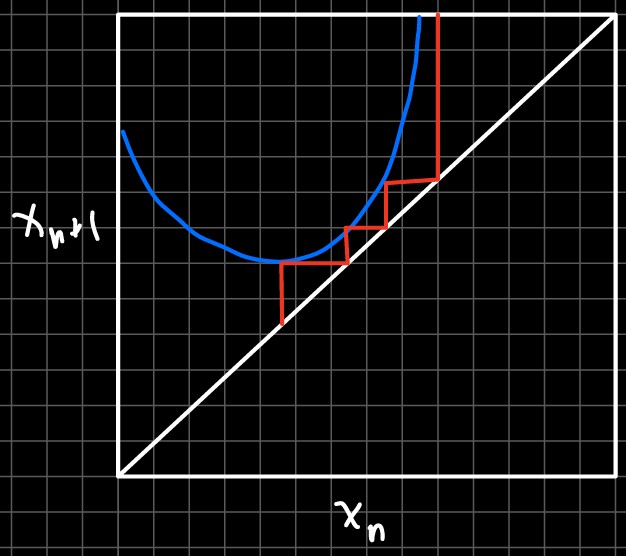
\includegraphics[width=\textwidth]{image copy.png}
		\caption{Cobweb diagram for \(c=0.4\)}
	\end{subfigure}
	\begin{subfigure}{0.48\textwidth}
		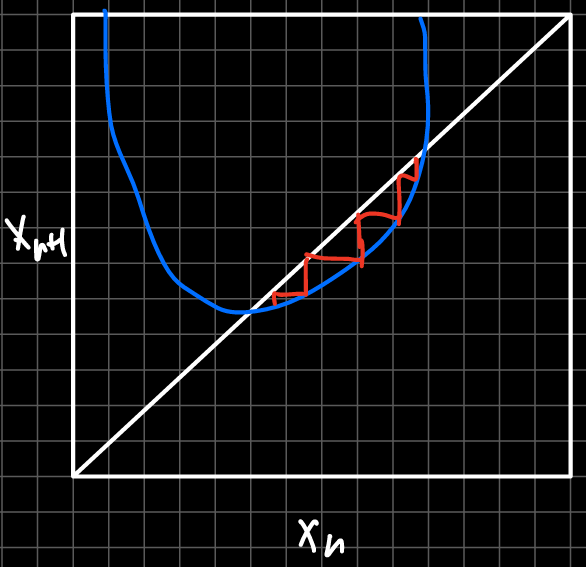
\includegraphics[width=\textwidth]{image copy 2.png}
		\caption{Cobweb diagram for \(c=0\)}
	\end{subfigure}
\end{figure}
On the left cobweb, we can see that the behavior is unbound and will tend to infinity. On the right cobweb, \(x=1\) is a source and \(x=0\) is a stable sink. points beyond \(x=1\) will go to infinity. points before \(x=0\) will converge to \(x=0\).
\subsection{Fixed points and Stability}
To find the fixed points we solve 
\begin{equation}
	x^2-x+c=0
\end{equation}
whose solutions are 
\begin{equation}
	x_{\pm} = \frac{1\pm\sqrt{1-4c}}{2}
\end{equation}
looking at the derivative at those points and restricting to only real values
\begin{align}
	f'(x_\pm)=1\pm\sqrt{1-4c} = \begin{cases}
		f'(x_+) = 1+\sqrt{1-4c} \geq 1 \\
		f'(x_-) = 1-\sqrt{1-4c}
	\end{cases}
\end{align}
to check the second point's stability we require that 
\begin{equation}
	-1 < 1-\sqrt{1-4c} < 1
\end{equation}
which is satisfied for 
\begin{equation}
	-\frac{3}{4} < c < \frac{1}{4}
\end{equation}
in summary, \(x_+\) is always unstable, and \(x_-\) is stable for \(-\frac{3}{4} < c < \frac{1}{4}\).
\subsection{Bifurcations and Types}
Using the last section we see two points:
\begin{enumerate}
	\item \(c=\frac{1}{4}\). Both fixed points combine and disappear for \(c>\frac{1}{4}\). When that happens the derivative is exactly \(+1\) so the graph of \(f\) is tangent to the diagonal, meaning this is a tangent bifurcation.
	\item \(c=-\frac{3}{4}\). No new fixed point is created so this ia a period-doubling bifurcation.
\end{enumerate}
\subsection{period-2 orbit}
period-2 points are where \(f^2(x)=x\) so in our case 
\begin{equation}
	0=\ins{x^2+c}^2+c-x = x^4 +2cx^2 -x +c^2 +c=0
\end{equation}
but since we have two fixed points from the original \(f(x)\) we can treat them as solutions and factor them out using polynomial division giving
\begin{equation}
	f^2(x)-x = \ins{x^2-x+c}\ins{x^2+x+c+1}
\end{equation}
which means the 2-cycle is the roots of the second element 
\begin{equation}
	p,q = \frac{-1\pm\sqrt{-4c-3}}{2}
\end{equation}
we can notice that for \(c=-\frac{3}{4}\) both roots coincide meaning the 2-orbit emerges from the fixed point associated with that value of c.
\subsection{Stability range}
Taking the derivative
\begin{equation}
	(f^2)'(p) = f'(f(p))\cdot f'(p) = f'(q)\cdot f'(p) = 4pq
\end{equation}
then using Vieta on the second element we have 
\begin{equation}
	pq = c+1
\end{equation}
so the multiplier is 
\begin{equation}
	\mu = 4c+4
\end{equation}
and to have stability 
\begin{equation}
	-1 < 4c+4 < 1 \implies -\frac{5}{4}<c<-\frac{3}{4}
\end{equation}
\subsection{bifurcation diagram}
\begin{figure}[h]\centering
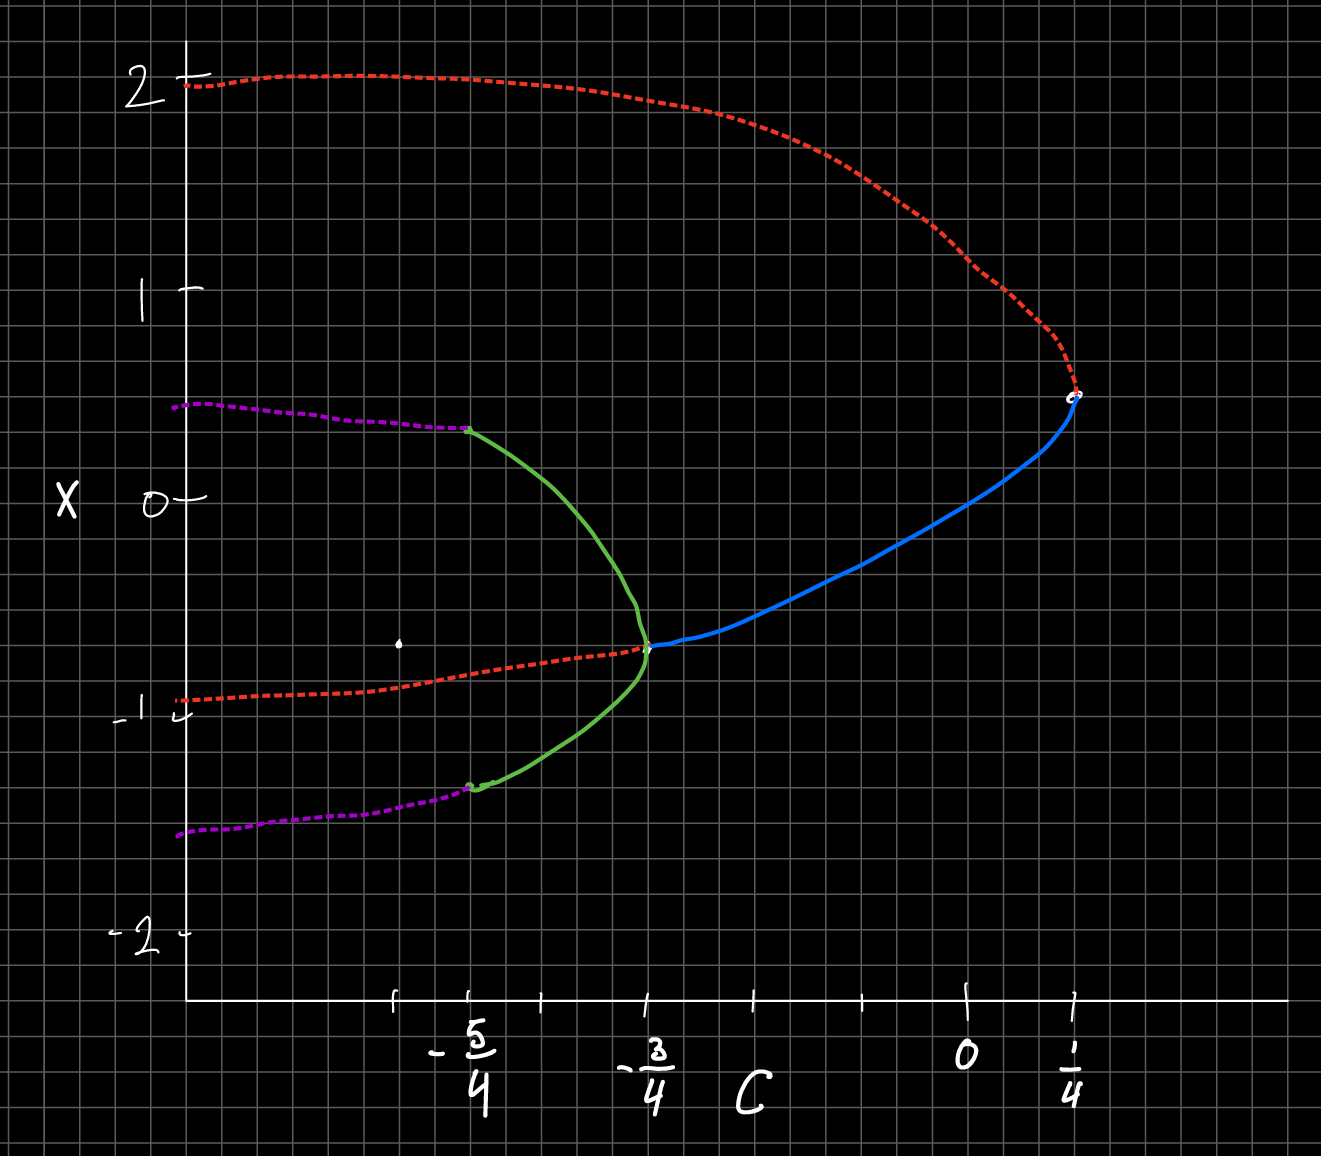
\includegraphics[width=0.75\textwidth]{image.png}
\caption{bifurcation diagram. Solid lines are stable, dashed are unstable. The tangent bifurcation is seen at \(c=0.25\), and the flip at \(c=-0.75\). At \(c=-1.25\) the 2-cycle destabilises.}
\end{figure}